\documentclass{tufte-handout}

%\geometry{showframe}% for debugging purposes -- displays the margins

\usepackage{amsmath}

% Set up the images/graphics package
\usepackage{graphicx}
\setkeys{Gin}{width=\linewidth,totalheight=\textheight,keepaspectratio}
\graphicspath{{graphics/}}

\title{Hierarchical approach for determining distribution of parameters consistent with experiments measuring transport of water in PMMA}
\author[]{}
%\date{}  % if the \date{} command is left out, the current date will be used

% The following package makes prettier tables.  We're all about the bling!
\usepackage{booktabs}

% The units package provides nice, non-stacked fractions and better spacing
% for units.
\usepackage{units}

% The fancyvrb package lets us customize the formatting of verbatim
% environments.  We use a slightly smaller font.
\usepackage{fancyvrb}
\fvset{fontsize=\normalsize}

% Small sections of multiple columns
\usepackage{multicol}

% Provides paragraphs of dummy text
\usepackage{lipsum}

% These commands are used to pretty-print LaTeX commands
\newcommand{\doccmd}[1]{\texttt{\textbackslash#1}}% command name -- adds backslash automatically
\newcommand{\docopt}[1]{\ensuremath{\langle}\textrm{\textit{#1}}\ensuremath{\rangle}}% optional command argument
\newcommand{\docarg}[1]{\textrm{\textit{#1}}}% (required) command argument
\newenvironment{docspec}{\begin{quote}\noindent}{\end{quote}}% command specification environment
\newcommand{\docenv}[1]{\textsf{#1}}% environment name
\newcommand{\docpkg}[1]{\texttt{#1}}% package name
\newcommand{\doccls}[1]{\texttt{#1}}% document class name
\newcommand{\docclsopt}[1]{\texttt{#1}}% document class option name

\begin{document}

\maketitle% this prints the handout title, author, and date

%\begin{abstract}
%\noindent This document describes the Tufte handout \LaTeX\ document style.
%It also provides examples and comments on the style's use.  Only a brief
%overview is presented here; for a complete reference, see the sample book.
%\end{abstract}

%\printclassoptions


\section{Experimental Data}
The available experiments measure the `water vapor transport rate', or the flux
of water through a nominally 1D geometry of the test sample. The experiment
begins by establishing a `dry' sample by flowing dry air through the
measurement chambers, then switches to a fixed temperature and relative
humidity on one side of the sample. The other side of the sample is maintained
at $\sim 0\%$ relative humidity and the flux of water out of the sample is
measured. An analytic solution is available. The model is:
\begin{marginfigure}%
    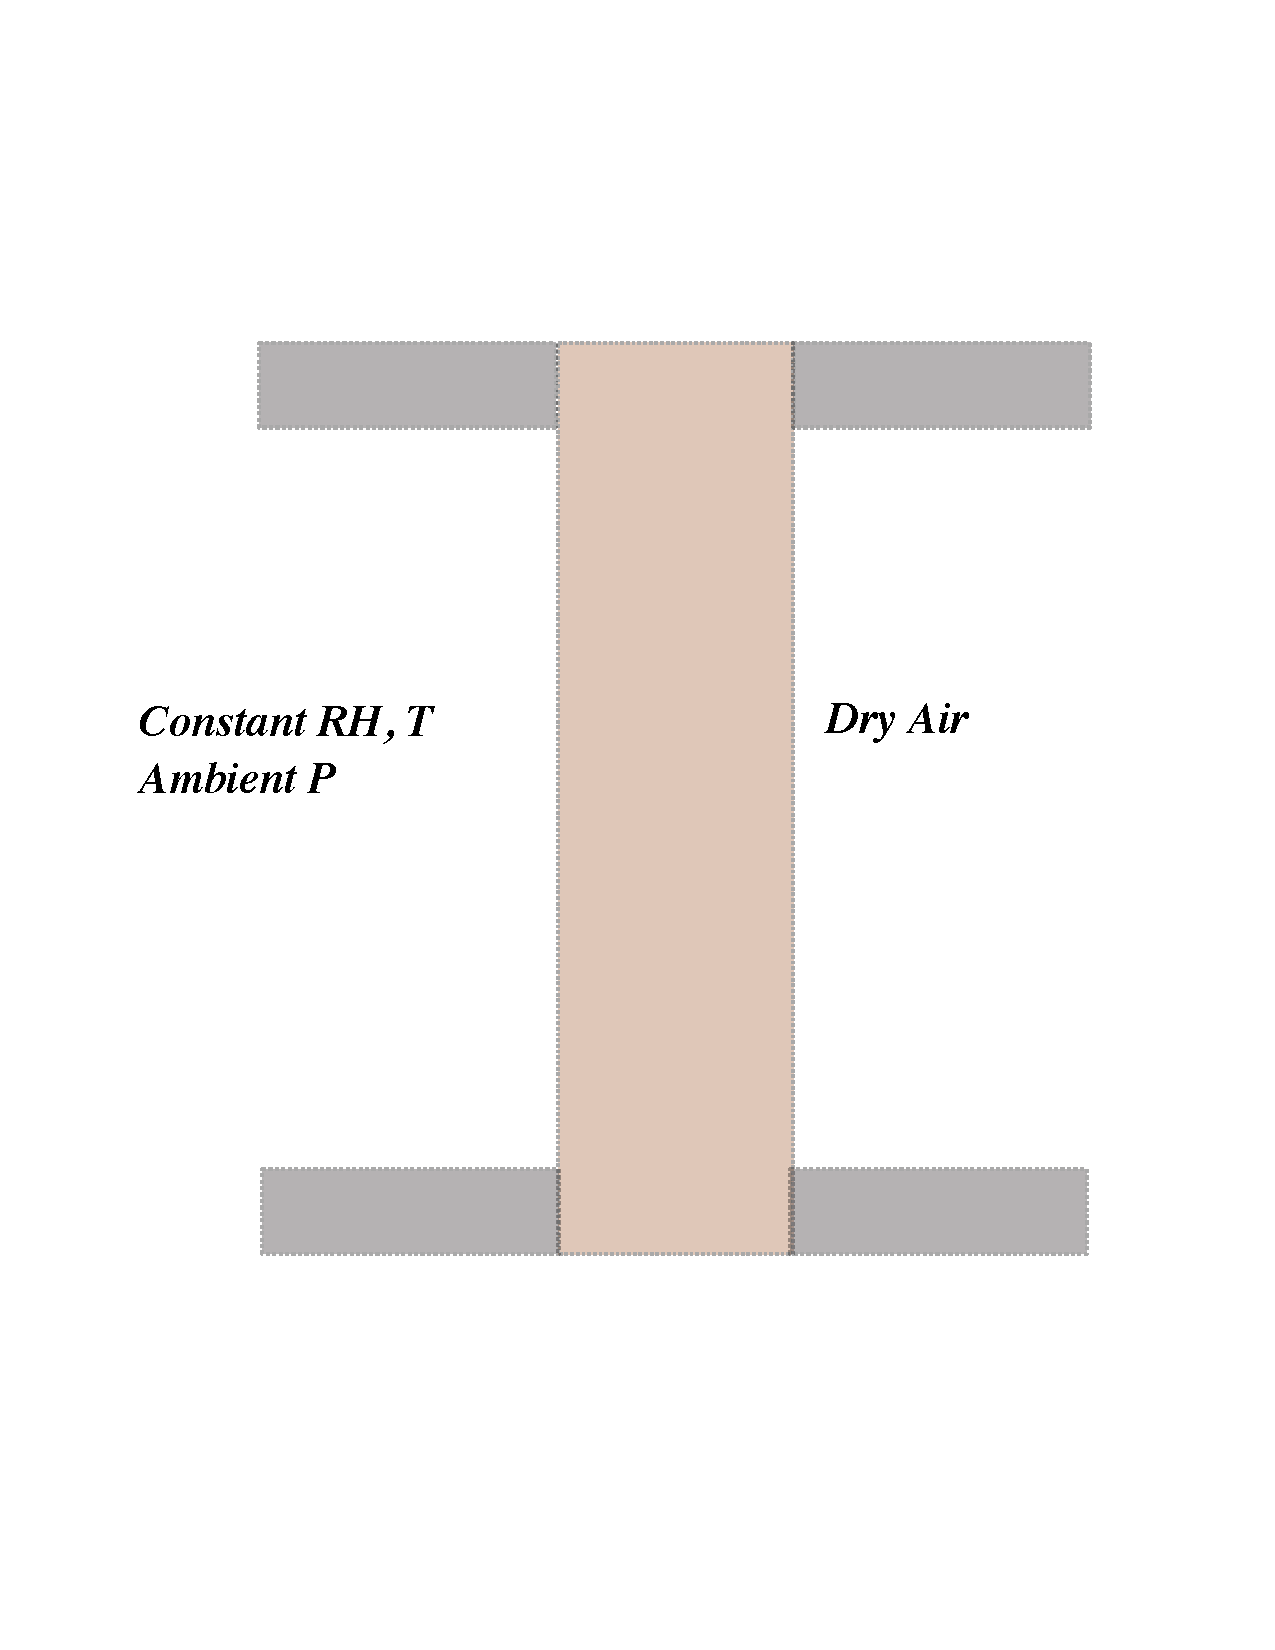
\includegraphics[width=1.0\linewidth]{WVTR.pdf}
    \caption{
    Measurements taken with MOCON Permatran; output of experimental measurement
is time trace of water vapor transport rate }
    \label{fig:marginfig}
\end{marginfigure}

\begin{equation} \frac{\partial C}{\partial t} =
    \frac{\partial}{\partial x} D \frac{\partial C}{\partial x}
\end{equation}

\begin{itemize}
  \item Dirichlet boundary conditions:
      \begin{itemize}
          \item $C=k_Da$ at $x=0$
          \item $C=0$ at $x=L$
          \item $a$ is activity; $a = (RH)\left.\frac{P_{\mathrm{sat}}}{P_{\mathrm{a}}}\right|_{T_\mathrm{amb}}$
        \end{itemize}
   \item Closed form solution 
       \begin{equation}
           \mathrm{WVTR} = \frac{DKa}{L}\sum_{n=0}^{\infty} 2(-1)^ne^{-Dn^2\pi^2(t-t_0)/l^2}
       \end{equation}
\end{itemize}

Both parameters ($D,K$) have an exponential temperature dependence.
\begin{gather}
        D = D_0 e^{D_1/T}\\
        K = K_0 e^{K_1/T}
\end{gather}
Four experiments are available at various temperatures. 

\section{Normalizing experimental data}
\newthought{The experiments should have the same importance}, or at least they
should not have different influence simply due to the number of data points
extracted. Scaling the probabilities by raising the probability for a each
experiment to the $\frac{1}{N}^{th}$ power, where $N$ is the number of sample
points is the current approach to address this. That is, for the lnlikihood for
$M$ experiments with $N_m$ datapoints
\begin{equation}
    F_D = \sum_{m=1}^{M} \left[ -0.5\frac{1}{N_m} \sum_{n=1}^{N_m} (f_{m,n}^{\mathrm{model}} - f_{m,n}^{\mathrm{measured}})^2 \frac{1}{\sigma_{m,n}^2} \right]
\end{equation}


\section{ToDo List}
\newthought{The premise} is that model for experiment \#2 is more expensive
than \#1, and we are conducting an experiment to see if we can reduce the
number of evaluations of the model for \#2 by using a hierarchical approach.
\begin{enumerate}
    \item Run emcee sampler on $p(\phi|Z_1,Z_2)$, that is, using all of the
        experimental data for a `large' number of samples. This will serve as
        `ground truth', with large being $\sim 4(10^6)$ per walker (8 walkers).
        Initial walker positions in a small ball around the MLE.
    \item Run emcee sampler on experiment \#1 only, to determine $p(\phi|Z_1)$.
        Do this several times in sequence, each time drawing the initial walker
        positions from the prior. Take `many' (e.g., 4M) samples. For the first
        attempt, use a very broad prior to draw samples for initial walker
        position.\footnote{This is a bit contrived, but the supposition is that
        we are not able to determine the MLE solution. So we are using sampling
    to reduce the space with each successive run and are putting the walkers in
a better position.}
    \item Sample the final posterior from experiment \#1 to get initial walker
        positions for the next step. Also bin the posterior samples to obtain a
        representation of the distribution $\mu_{H}^1(D_0,D_1,K_0,K_1|Z_1)$
        that can be evaluated at an arbitrary $(D_0,D_1,K_0,K_1)$.
    \item Run the emcee sampler on $p(\phi|Z_1,Z_2)$, but this time use initial
        walker positions obtained through consideration of Experiment \#1, and
        use $\mu_H^1$ as the prior\footnote{Using the prior facilitates an optimization where we don't bother evaluating the sample if the prior is $< p_{min}$}. Compare the posterior to the baseline
        posterior obtained in the first step.  Take fewer (e.g., 100k) samples. 
    \item Run the emcee sampler on $p(\phi|Z_2)$, using $\mu_H$ as a prior.
        Compare the posterior to the baseline posterior from the first step.
    \item Redo the first step, but use only the number of samples corresponding
        to the number of function evaluations for Expt. \#2 in the hierarchical
        approach.
    \item Alternatively, everywhere emcee sampler is used, attempt GD
        optimization starting from the walker positions, and if successful use
        IS in place of emcee sampler. 
\end{enumerate}


\bibliography{sample-handout}
\bibliographystyle{plainnat}



\end{document}
